\subsubsection{Mudança de Altitude (Altitude Change)}

Neste cenário de mudança de altitude, o objetivo é que o drone ajuste sua altura em resposta a uma nova referência de altitude, mantendo-se estável nas posições \(X\) e \(Y\) durante essa mudança. Além de analisar o desempenho do controlador de altitude, também é importante observar como os controladores de posição e atitude reagem a essa transição.

Parâmetros da simulação: \\

- Tempo total: 25 segundos;\\
- Altura inicial: 2 metros; \\
- Altura desejada: 1 metros; \\
- Posição em \(X\) e \(Y\): 0, 0. \\
- t mudança de altitude: 2s



1) Coordenada Z

O gráfico abaixo mostra o comportamento da coordenada \(Z\) ao longo do tempo.

\begin{figure}[H]
	\centering
	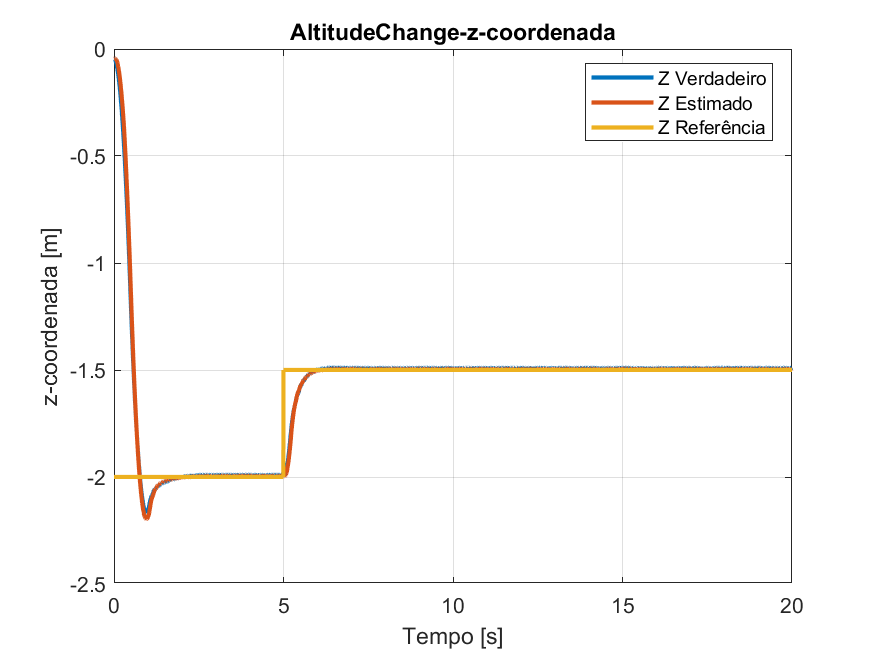
\includegraphics[width=1\textwidth]{AltitudeChange-z-coordenada.png}
	\caption{Coordenada Z para o Cenário de Mudança de Altitude}
	\label{fig:altitudechange-z-coordenada}
\end{figure}

Observamos que o sistema atinge a nova referência de altitude rapidamente, com um pequeno overshoot após a mudança de altitude. A estabilização ocorre após aproximadamente 5 segundos. Esse comportamento indica um bom desempenho do controlador de altitude para alcançar o valor de referência com um erro em regime permanente praticamente nulo.

2) Coordenadas X e Y

Os gráficos a seguir mostram o comportamento das coordenadas \(X\) e \(Y\) ao longo do tempo, permitindo uma análise do controle de posição durante a mudança de altitude.

\begin{figure}[htbp]
    \centering
    \subfloat[Coordenada X para o Cenário de Mudança de Altitude]{
        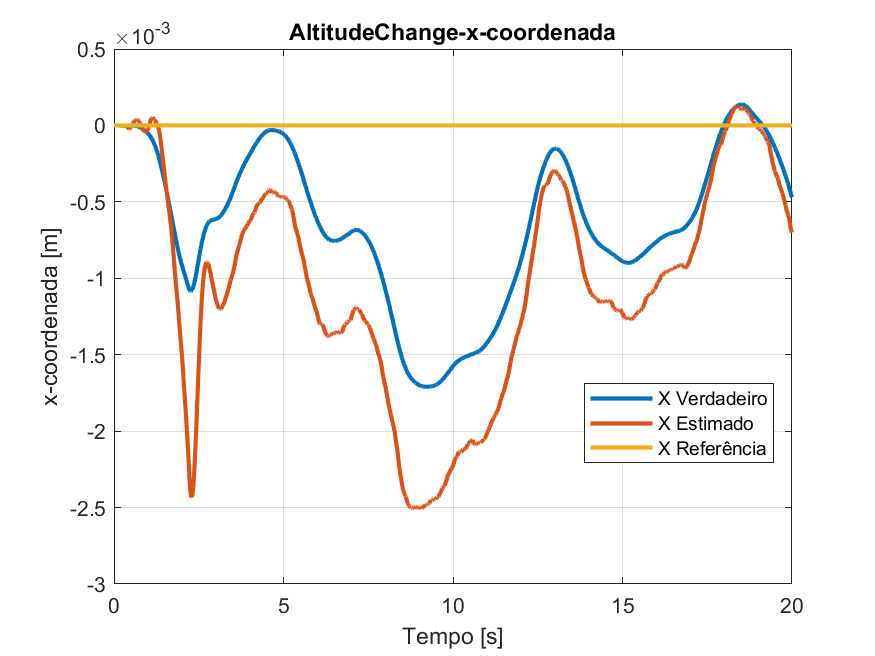
\includegraphics[width=0.45\textwidth]{AltitudeChange-x-coordenada.png}
        \label{fig:altitudechange-x-coordenada}
    }
    \hfill
    \subfloat[Coordenada Y para o Cenário de Mudança de Altitude]{
        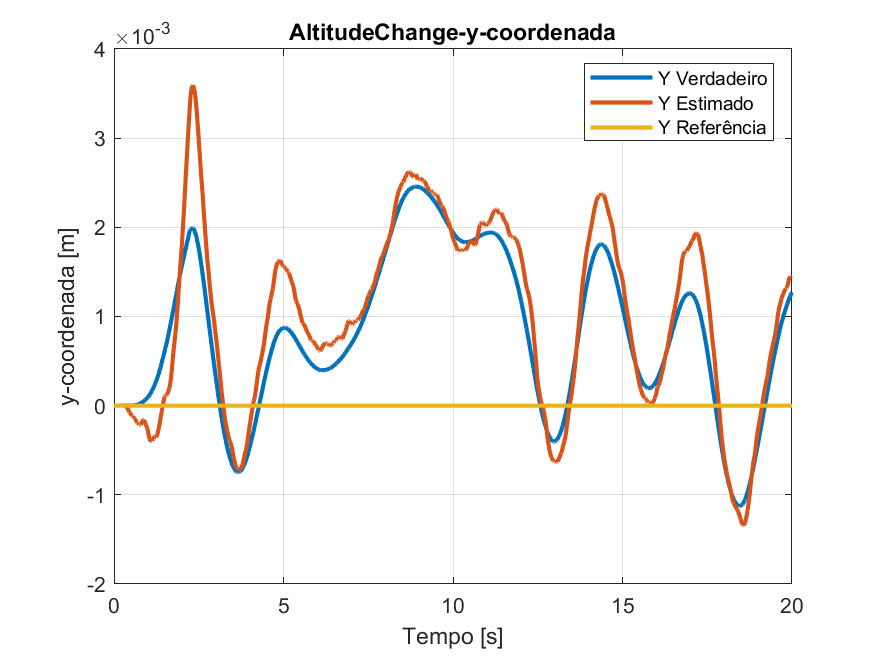
\includegraphics[width=0.45\textwidth]{AltitudeChange-y-coordenada.png}
        \label{fig:altitudechange-y-coordenada}
    }
    \caption{Coordenadas X e Y para o Cenário de Mudança de Altitude}
    \label{fig:altitudechange-x-y-coordenadas}
\end{figure}

Nos gráficos das coordenadas \(X\) e \(Y\), observamos que, durante a mudança de altitude, as posições \(X\) e \(Y\) nâo exibem oscilações significativas, na ordem dos milímetros, em torno da posição de referência. A curva de estimativa de posição \(Y\) (linha laranja) tem uma amplitude de oscilação baixa em comparação com a curva verdadeira e podemos ver que a amplitiude diminui com o tempo. No gráfico de \(X\), o comportamento é semelhante, com oscilações que diminuem progressivamente em direção a estabilidade.

Essas oscilações mostran que o sistema de controle de posição consegue manter a estabilidade durante a transição de altitude. Sendo interessante notar que o sistema de comporta melhor após a mudança de altitude do que num voo pairado, sendo assim, ao realizar nossos ajustes no sistema para melhorar o desempenho em voo pairado, devemos tomar cuidado para não prejudicar o sistema em um cenário de mudança de altitude..

3) Ângulos de Rolagem, Arfagem e Guinada

Os gráficos a seguir mostram os ângulos de rolamento (roll), arfagem (pitch) e guinada (yaw) do quadricóptero durante a mudança de altitude.

\begin{figure}[htbp]
    \centering
    \subfloat[Arfagem para o Cenário de Mudança de Altitude]{
        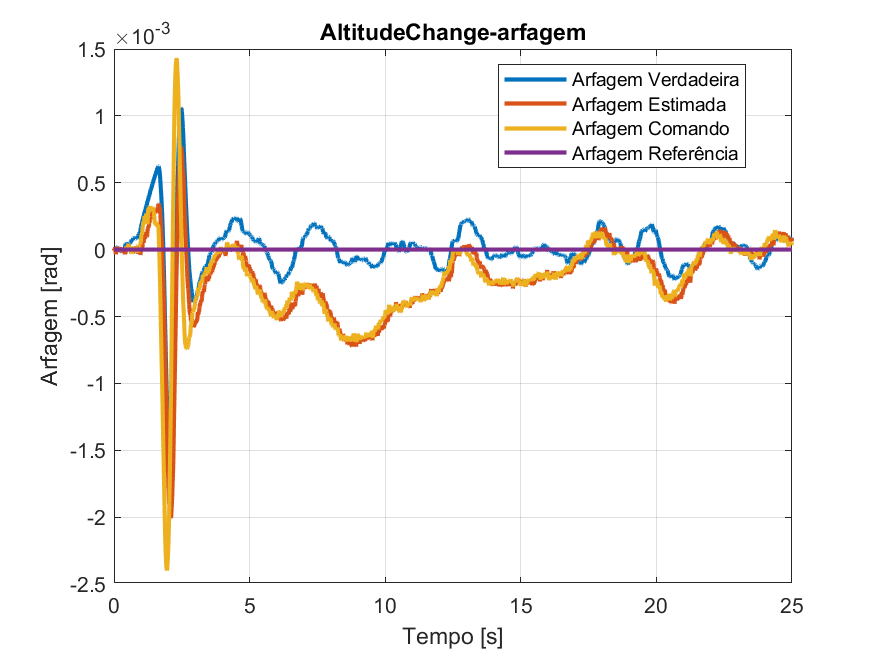
\includegraphics[width=0.45\textwidth]{AltitudeChange-arfagem.png}
        \label{fig:altitudechange-arfagem}
    }
    \hfill
    \subfloat[Guinada para o Cenário de Mudança de Altitude]{
        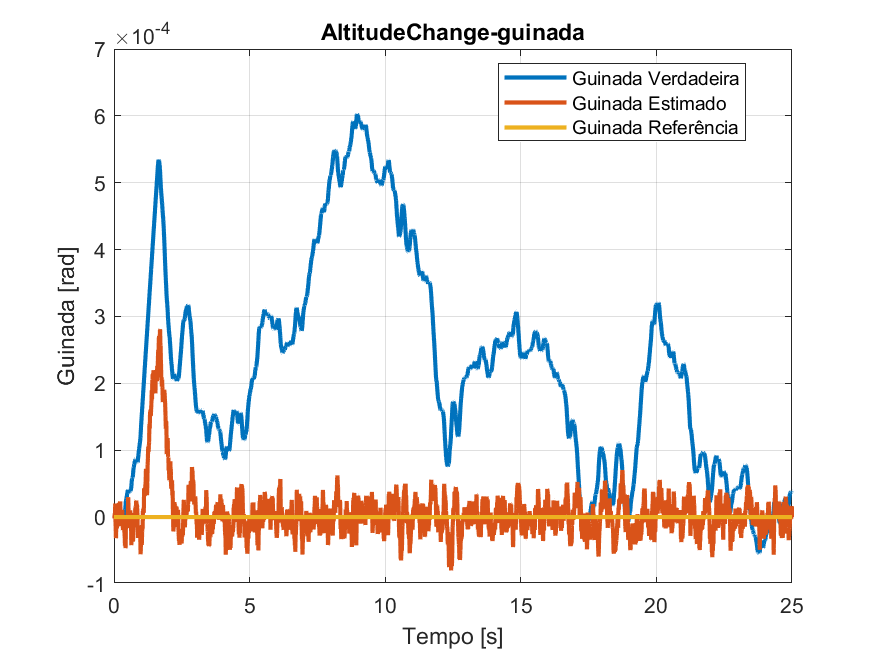
\includegraphics[width=0.45\textwidth]{AltitudeChange-guinada.png}
        \label{fig:altitudechange-guinada}
    }
    \caption{Arfagem e Guinada para o Cenário de Mudança de Altitude}
    \label{fig:altitudechange-arfagem-guinada}
\end{figure}

\begin{figure}[H]
	\centering
	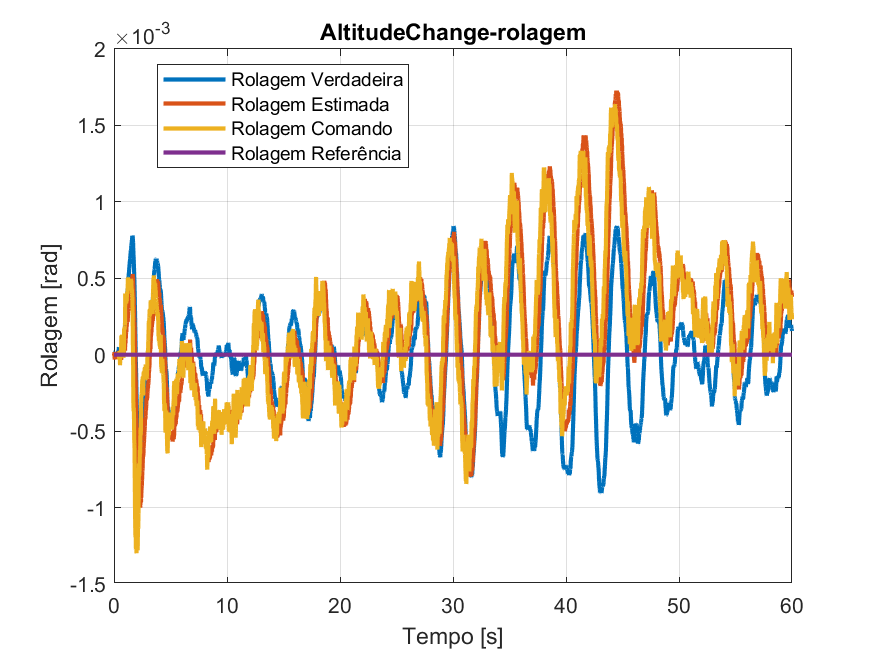
\includegraphics[width=0.5\textwidth]{AltitudeChange-rolagem.png}
	\caption{Rolagem para o Cenário de Mudança de Altitude}
	\label{fig:altitudechange-rolagem}
\end{figure}

Durante a transição de altitude, os ângulos de arfagem e rolamento apresentam oscilações notáveis, mas de baixa amplitude. No gráfico de arfagem e de rolagem, observa-se um comportamento oscilatório acentuado no momento da mudança de altitude,mas que com o tempo tende a estabilidade em torno do valor de referência, o que indica que o controlador precisa ser ajustado para responder de forma mais suave. O gráfico de guinada mostra variações menores, o que sugere um controle mais estável para esse eixo.

%A amplitude das oscilações em rolamento e arfagem indica que o sistema de controle está mal ajustado para esses eixos durante a transição de altitude. Ajustes nos parâmetros de controle, como o ganho derivativo \(K_d\), poderiam ajudar a reduzir essas oscilações e melhorar a resposta do sistema.

%### Conclusão Geral para o Cenário de Mudança de Altitude

%No cenário de mudança de altitude, o controlador de altitude funciona bem, atingindo o novo valor de referência de forma rápida e com mínimo erro em regime permanente. No entanto, os controladores de posição nos eixos \(X\) e \(Y\) e os controladores de atitude nos eixos de rolamento e arfagem exibem sinais de instabilidade, com oscilações crescentes ao longo do tempo. Para melhorar o desempenho, recomenda-se um ajuste nos ganhos do controlador, especialmente nos eixos \(X\) e \(Y\), bem como nos controladores de atitude, para reduzir as oscilações e melhorar a estabilidade geral do sistema.


%---------------------------------------------------------------------
% INDICE REMISSIVO
%---------------------------------------------------------------------
\phantompart
\printindex
%---------------------------------------------------------------------
